\subsection{Receiver Executor communication}

Dieses Sequenzdiagramm beschreibt am Beispiel des CommandExecutors und des TruffleReceivers, wie das Notification Framework funktioniert.
Beide Services laufen in verschiedenen Threads. Der CommandExecutor nimmt solange Commands von seinen Queues, bis keine abzuarbeitenden
Commands mehr vorhanden sind. Falls dieser Fall eintreten sollte, so wird der thread schlafen gelegt, bis ein neues Element auf eine
der Queues geschrieben wird. Parallel dazu empfängt der TruffleReceiver von Snort Paketdaten und packt diese in Truffle. Anschließend
wird ein AddPacketDataCommand erstellt und das Truffle übergeben. Der Command wird dann mittels der receive Methode des CommandExecutor listeners
an diesen übergeben. Die receive Methode schreibt dann intern auf die CommandQueue des CommandExecutors. Dadurch wird dieser wieder aufgeweckt,
um die neuen Commands abzuarbeiten.

\FloatBarrier
\begin{sidewaysfigure}
  \centering
  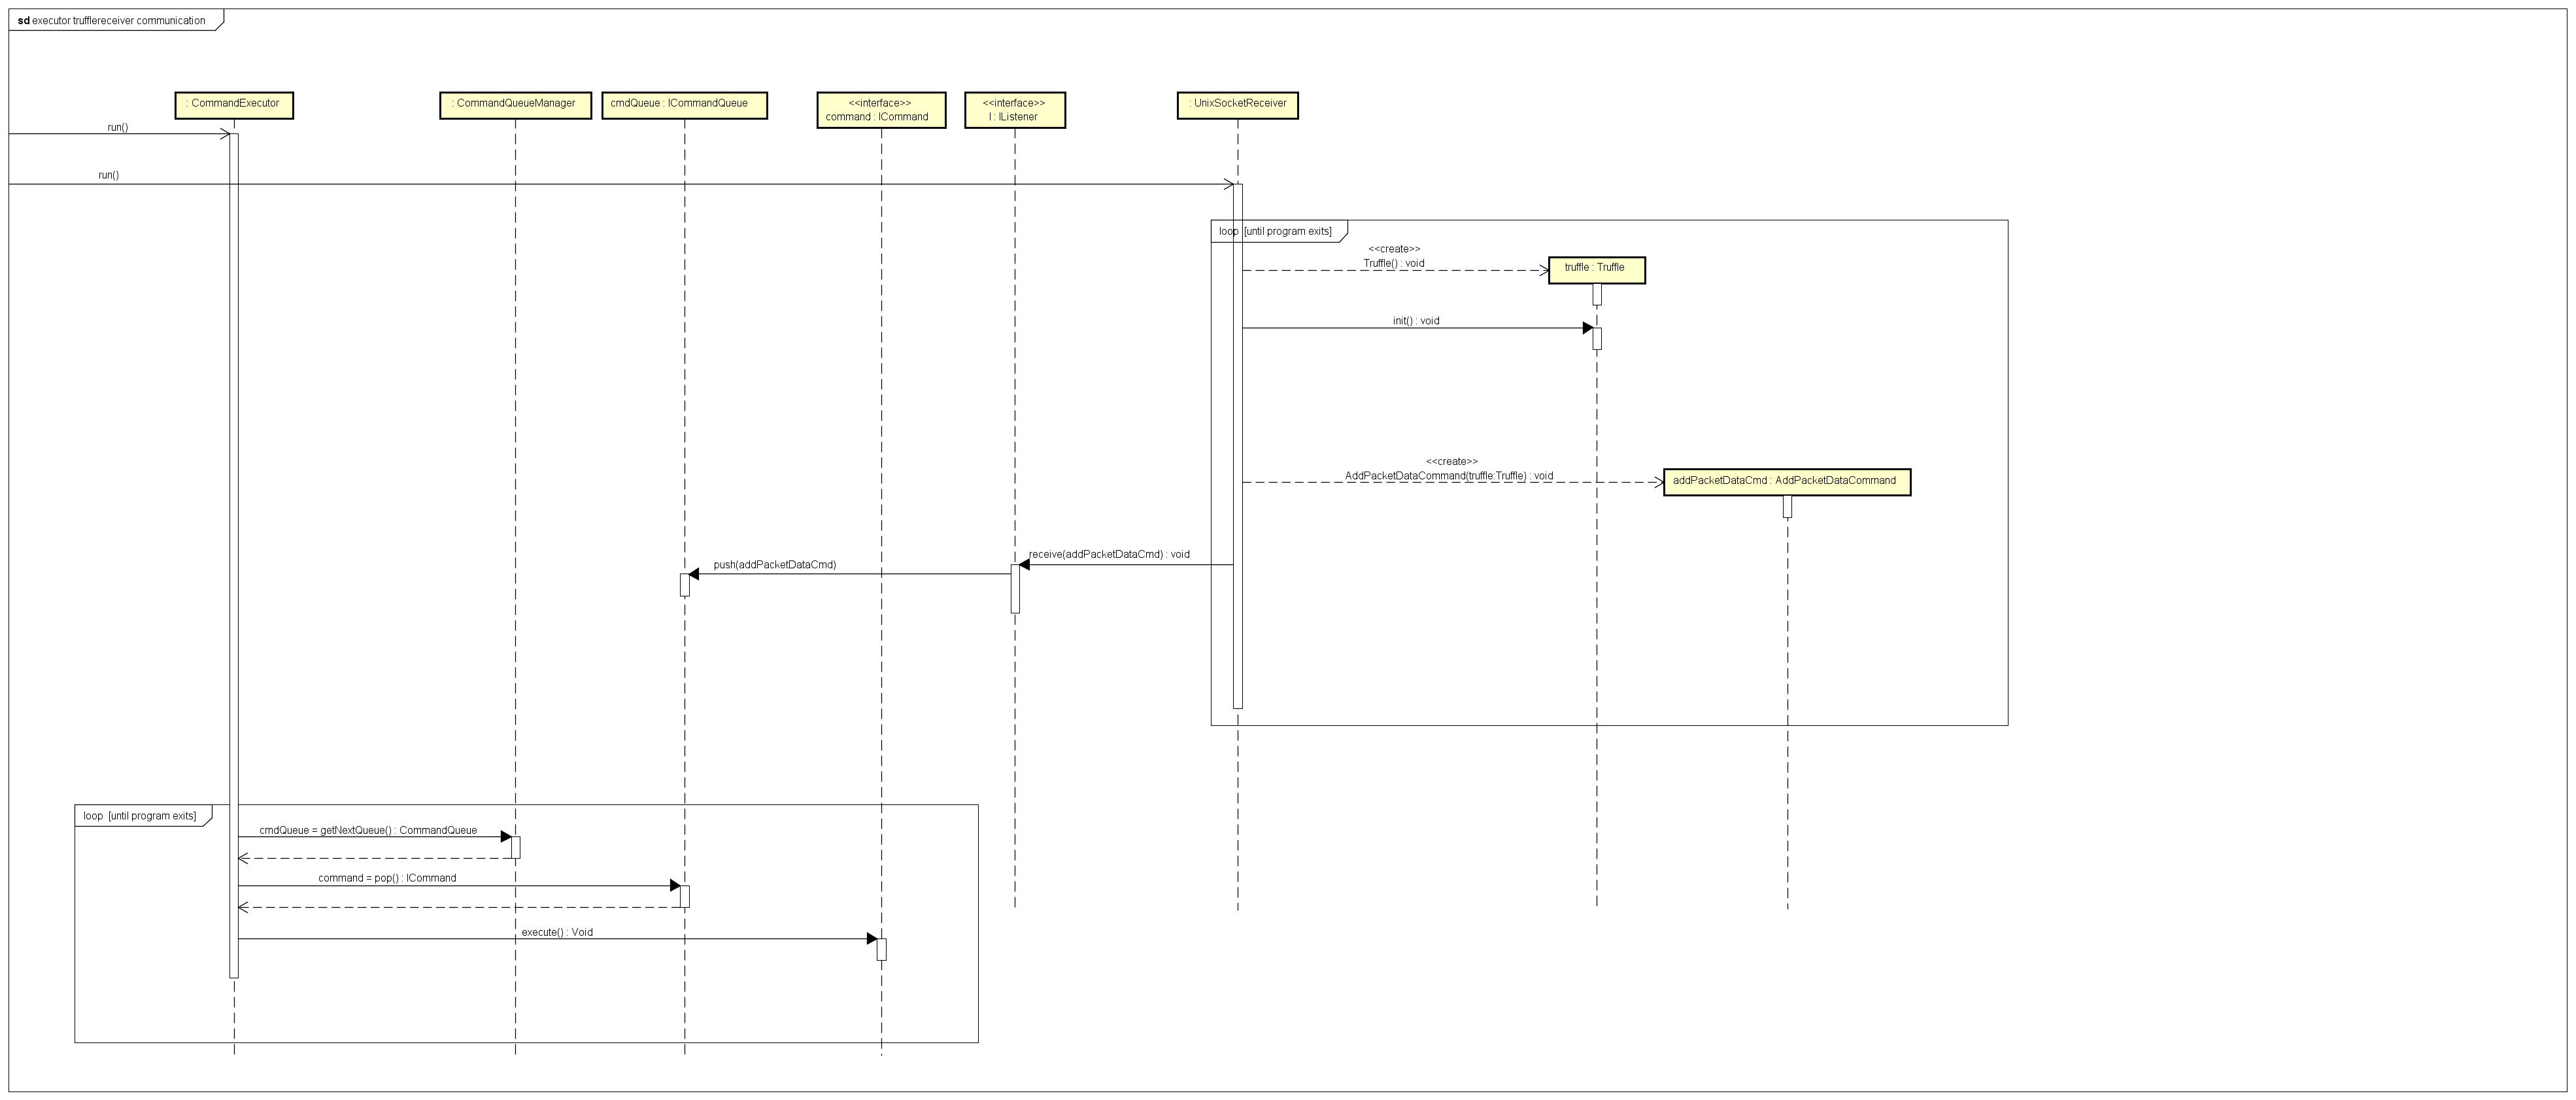
\includegraphics[width=\textwidth]{../diagramimages/sd_receiver_executor_comm.png}
  \caption[Sequenzdiagramm Receiver Executor communication]{Sequenzdiagramm Receiver Executor communication}
\end{sidewaysfigure} \FloatBarrier 